\documentclass{article}
\usepackage{tikz}
\usepackage{amsmath, empheq}
\begin{document}
    % TikZ picture with origin upper left
    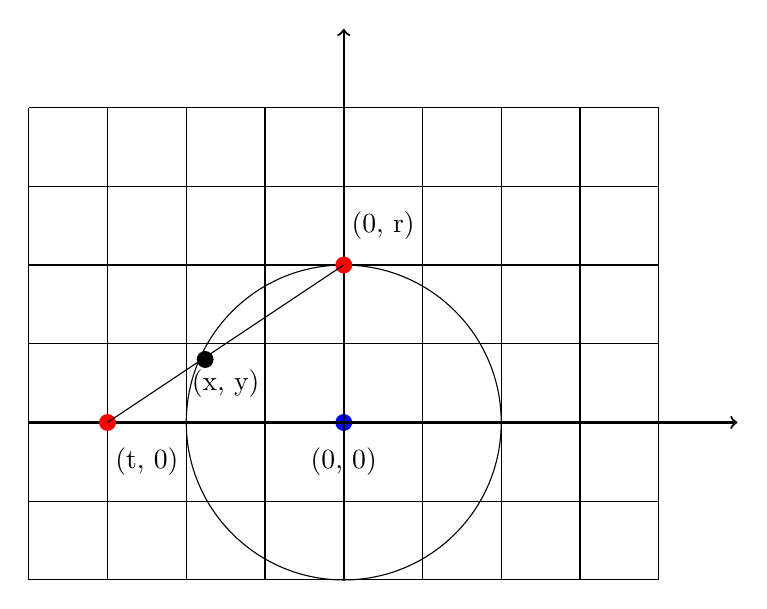
\begin{tikzpicture}[yscale=-1] 
        % 4x4 grid
        \draw (-2, 0) grid (6, 6);
        % origin point
        \draw [color=blue, fill=blue] (2, 4) circle (0.1);
        % x-axis
        \draw [thick,->] (-2, 4) -- (7, 4);
        % y-axis
        \draw [thick,->] (2, 6) -- (2, -1);
        % origin label
        \node at (2, 4.5) {(0, 0)};
        \draw (2, 4) circle (2);
        \draw [color=red, fill=red] (2, 2) circle(0.1);
        \node at (2.5, 1.5){(0, r)};
        \draw [color=red, fill=red] (-1, 4) circle(0.1);
        \node at (-0.5, 4.5){(t, 0)};
        \draw (2, 2)--(-1, 4);
        \node at (0.5, 3.5){(x, y)};
        \draw [color=black, fill=black] (0.24, 3.2) circle(0.1);
    \end{tikzpicture}\\ \\
	\centerline{Derive circle parametric equation}
\end{document}
